\documentclass{article}

\usepackage{epsfig}
\usepackage[export]{adjustbox}% http://ctan.org/pkg/adjustbox
\usepackage{caption}
\usepackage{subcaption}
\usepackage{fullpage}
\usepackage{commath}
\usepackage{amssymb}
\usepackage[space]{grffile}
\usepackage{float}

\def\E{\mathbb{E}}
\def\R{\mathbb{R}}
\def\bin{\text{bin}}
\def\bet{\text{beta}}
\def\Bin{\text{Binom}}
\def\diag{\text{diag}}

\title{Single Sequence HMM in DNA Methylation Problem}
\author{Chicheng Zhang}

\begin{document}
\maketitle

\section{The Model}

In the problem of DNA methylation, we are given a sequence $\cbr{x_t = (c_t, \mu_t)}_{t=1}^l$, where at each time $t$, the coverage is an nonnegative integer $c_t \in \cbr{0,1,\ldots,N}$ and the methylation count is $\mu_t \in \cbr{0,1,\ldots,c_t}$. We model the data using a hidden Markov model, that is, the underlying dynamics of the hidden states is driven by a Markov chain $\cbr{h_t}$, where $h_t \in [m]$. We leave the consideration of context information to the next stage.

The HMM can be summarized by parameters $(\pi, T, O)$, where $\pi \in \R^m$ is the initial probability distribution $\Pr(h_1)$ and $T \in \R^{m \times m}$ is the transition matrix of the Markov chain $\Pr(h_{t+1} | h_t)$, $O$ is the observation matrix, namely the conditional probability of methylation and coverage, given hidden state $\Pr(c_t, \mu_t | h_t)$. To avoid notation clutter, we drop the time indices $t$ if they are the same among all the variables appeared in a formula.

We assume the $\mu_t$ given $c_t$ and $h_t$ is drawn from a binomial distribution, and for each hidden state $h \in [m]$ there is a methylation probability $p_h \in [0,1]$ associated with it. Formally,
\[ \mu_t | c_t, h_t \sim \Bin(c_t, p_{h_t}) \]

\section{Algorithm based on Method of Moments}

Given an observation $(c, \mu)$, we map it to a $n$-dimensional vector using feature mapping $\phi$. Generally speaking, different feature mappings have different properties.

For mapping $\phi$, we define the corresponding observation matrices as follows:
\[ O_{\phi}^s := \E[\phi(c_s,\mu_s) | h_2] \]
for $s = 1,2,3$, where $h_2$ is the hidden state at time 2. It is worth pointing out that $O_\phi$ contains information to recover the $p_h$'s, and since
\[ O_{\phi}^3 = O_{\phi}^2 T, \qquad O_{\phi}^1 = O_{\phi}^2 \diag(\pi) T^T \diag(T\pi)^{-1}\]
if we can recover $O_{\phi}^s$, $s = 1,2,3$, then we can recover $T$ and $\pi$ by algebra.

Conditional independence of $(c_1, \mu_1)$, $(c_2, \mu_2)$, $(c_3, \mu_3)$ given $h_2$ implies that
\[ \E[\phi(c_1, \mu_1) \otimes \phi(c_2, \mu_2) \otimes \phi(c_3, \mu_3)] = \sum_{i=1}^m w_i (O_{\phi}^1)_i \otimes (O_{\phi}^2)_i \otimes (O_{\phi}^3)_i \]
where $w_i = \Pr[h_2 = i] = (T\pi)_i$.
This tensor has a low rank structure.

Its empirical version can be computed by summing the outer products of mapped observation over training data; suppose the training data contains triples $\cbr{((c_{t,1}, \mu_{t,1}), (c_{t,2}, \mu_{t,2}), (c_{t,3}, \mu_{t,3}))}_{t=1}^{l}$, then
\[ \hat{\E}[\phi(c_1, \mu_1) \otimes \phi(c_2, \mu_2) \otimes \phi(c_3, \mu_3)] = \frac{1}{l} \sum_{t=1}^l \phi(c_{t,1}, \mu_{t,1}) \otimes \phi(c_{t,2}, \mu_{t,2}) \otimes \phi(c_{t,3}, \mu_{t,3}) \to \E[\phi(c_1, \mu_1) \otimes \phi(c_2, \mu_2) \otimes \phi(c_3, \mu_3)] \]

Therefore, applying CP-tensor decomposition on the empirical tensor gives an estimate of $O_{\phi}^s$, $s = 1,2,3$.


\section{Feature Maps}
Some examples of feature maps are given as follows.

\paragraph{Binning mapping} Given observation $(c, \mu)$, $\phi_{\bin, n}(c, \mu)$ is a $n$-dimensional vector, with its entries as follows:
\[ (\phi_{\bin, n}(c, \mu))_i = \begin{cases} I(\frac{\mu}{c} \in (\frac{i-1}{n}, \frac{i}{n}]) & c \neq 0 \\ 0 & c = 0 \end{cases} \]
where $n$ is a hyperparameter controlling the number of the bins, and the width of the bins is $\frac{1}{n}$.

\paragraph{Beta mapping} Given observation $(c, \mu)$, $\phi_{\bet, n}(c, \mu)$ is a $n$-dimensional vector, with its entries as follows:
\[ (\phi_{\bet, n}(c, \mu))_i = \frac{1}{B(\mu+1, c-\mu+1)} (\frac{i}{n})^\mu (1-\frac{i}{n})^{c-\mu} \]

\section{Experiment Results}
\subsection{Setting}
In this set of experiments, we focus on the methylation data in cell type E1 and chromosome 1.

Let $s$ be the number of base segments merged to a single segment. Specifically, we aggregate every $s$ observations to a single one. Namely, for all integers $k \geq 0$, we merge obervations $(c_{ks+1}, \mu_{ks+1})$, $(c_{ks+2}, \mu_{ks+2})$, \ldots, $(c_{ks+s}, \mu_{ks+s})$ to a single $(\tilde{c}_k, \tilde{\mu}_k)$, where
\[ \tilde{c}_k = \sum_{i=1}^k c_{ks+i}, \quad \tilde{\mu}_k = \sum_{i=1}^k \mu_{ks+i}\]
Note that the segments merged are non-overlapping.


Let $l$ be the length of the input sequence, that is, we draw $l$ 3-consecutive observations with replacement from the (merged) sequence $\cbr{(c_t, \mu_t)}_{t=1}^{L}$, forming a new dataset containing triples $\cbr{((\tilde{c}_{t,1}, \tilde{\mu}_{t,1}), (\tilde{c}_{t,2}, \tilde{\mu}_{t,2}), (\tilde{c}_{t,3}, \tilde{\mu}_{t,3}))}_{t=1}^{l}$.

Let $n$, the dimensionality of the feature mapping, be 30.

Let $m$ be the number of hidden states assumed. For example if $m = 4$, then the estimated matrix $O^2_{\phi} = \E[\phi(x)|h]$ has 4 columns.

%At this point we do not take into account the contexts, and we further assume that the coverage in different segments are non-uniform.

Although our ultimate goal is to recover the transition matrix and observation matrix of the hidden Markov model, at the current stage, we recover $\E[\phi(x)|h]$ for each value of $h$. Recall that $x = (c, \mu)$ is the (coverage, methylation) count pair in each segment. In the figures, the x-axis $t$ corresponds to the $i = (tn)^{\text{th}}$ coordinate of vector $\phi$. The $y$ axis corresponds to the values of $(\E[\phi(x)|h])_i$.


The value of $p_h$ for each $h$ can be straightforwardly extracted from $\E[\phi(x)|h]$. The transition matrix can also be computed subsequently. We leave the full recovery of the parameters to the next stage.

\paragraph{Recovery of $p_h$ from Expected Beta feature mapping}
Recall that
\[ \int_0^1 \frac{t t^{m}t^{c-m}}{B(m+1,c-m+1)} dt = \int_0^1 \frac{t t^{(m+1)-1}t^{(c-m+1)-1}}{B(m+1,c-m+1)} dt = \frac{m+1}{c+2} \]
Therefore,
\[ \int_0^1 \E[\phi(x,t) | h] dt = \E[\frac{m+1}{c+2} | h] = \E[\frac{cp_h + 1}{c + 2} | h] = \E[\frac{c}{c+2}] p_h + \E[\frac{1}{c+2}] \]
assuming independence between $h$ and $c$.
Let $a = \E[\frac{1}{c+2}]$. Then, $\int_0^1 \E[\phi(x,t) | h] dt = (1 - 2a) p_h + a$.
Hence,
\[ p_h = \frac{\int_0^1 \E[\phi(x,t) | h] dt - a}{1 - 2 a}. \]


%In subsequent results, we show the entire $\E[\phi(x)|h]$, as opposed to a single number $p_h \in [0,1]$. The reason is that we wish to recover more information about the hidden states learned, to get a better understanding of the HMM model.

%-- what features $\phi$ are you looking at?
%-- why are you showing the entire $\phi$ vector and not a single number?
%We focus on two types of feature mappings $\phi$, the first one is binning mapping:
%\[ \phi_{\bin}(x,y) = \begin{cases} {I(\frac{\mu}{c} \in (y,y+h])} & c \neq 0 \\ 0 & c = 0\end{cases} \]
%where $h$ is the width of the bins.

%The second one is Beta map:
%\[ \phi(x,y) = \frac{1}{B(\mu+1, c-\mu+1)}y^\mu (1-y)^{c-\mu} \]
%In this mapping there is no explicit notion of ``bin width", but the value of $c$ can be thought of as a parameter controlling it: if the coverage $c$ is large, then the bin width is small, and vice versa.

%In experiments, since it is impossible to write down $\E[\phi(x_1, \cdot) \otimes \phi(x_2, \cdot) \otimes \phi(x_3, \cdot)]$ and perform tensor decomposition, we use discretization: compute an empirical version of $\E[\phi(x_1, y_1) \otimes \phi(x_2, y_2) \otimes \phi(x_3, y_3)]$, where $y_1, y_2, y_3$ is in $\cbr{0,h,2h,\ldots,1}$. By decomposing this tensor we are able to recover $\E[\phi(x, y) | h]$, where $y$ is in $\cbr{0,h,2h,\ldots,1}$. By mild regularity assumption on the distribution of $x$, this can give a fairly accurate estimate of $\E[\phi(x, y) | h]$ where $y$ ranges in the $[0,1]$ interval.


\subsection{Effect of Sample Size $l$}
We fix $m = 4$, $s = 1$, and vary the sample size (number of triples collected) $l =$ 1000, 10000, 20000, 40000, 80000, 160000, 320000. The samples are drawn without replacement from the original dataset. Figure~\ref{fig:varyl} shows the result. Recall that the value of $m$ is the number of hidden states assumed; We observe that the output of the algorithm stablizes when $l \geq 80000$. \footnote{For the last few figures, although the colors of the lines in all subfigures are diffent, we observe that they have the same pattern.}

\begin{figure}[H]

    \begin{tabular}{cc}
    \begin{subfigure}[t]{0.45\textwidth}
        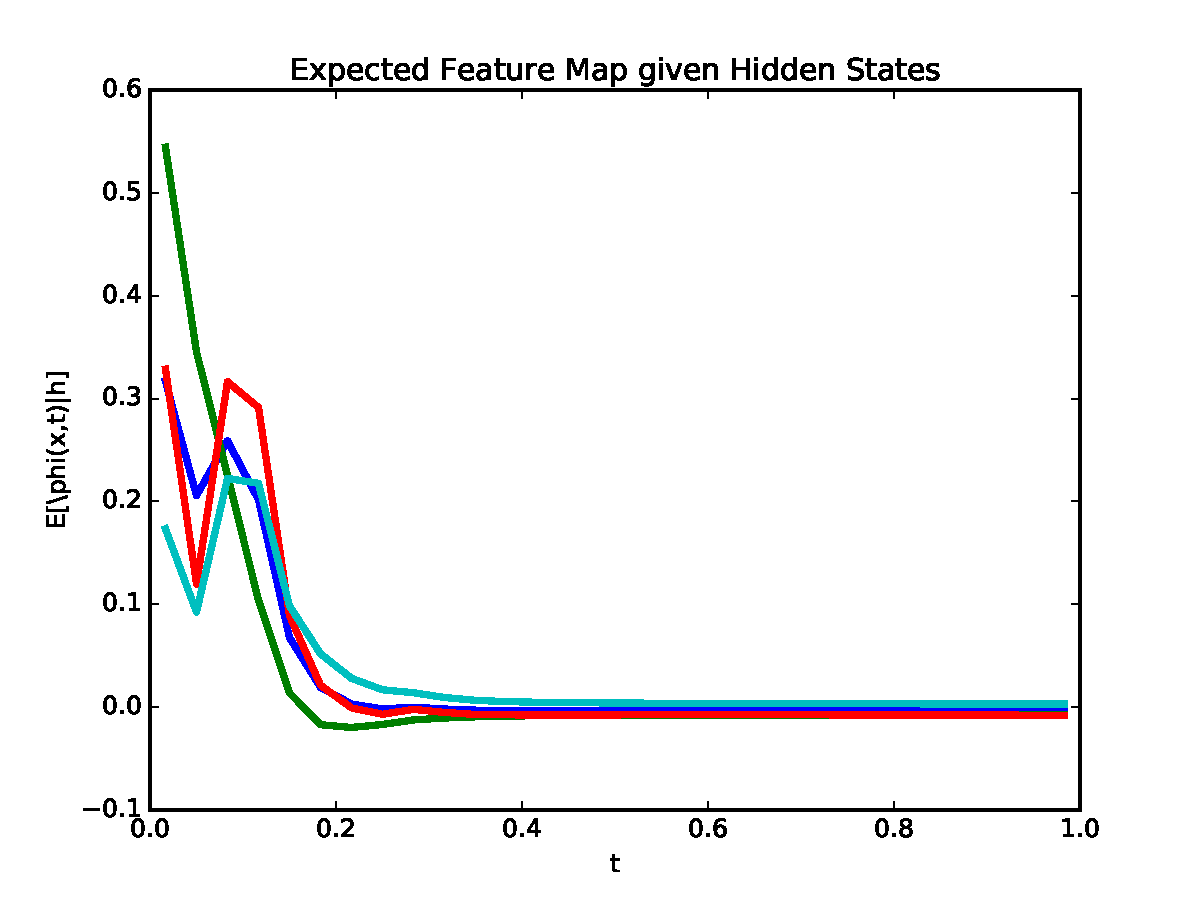
\includegraphics[width=\textwidth]{figs/vary_l/cell = E1_chr = 1_l = 10000_s = 1_m = 4_n = 30_phi = beta_full.pdf}
        \caption{$l = 10000$}
    \end{subfigure}
    &
    \begin{subfigure}[t]{0.45\textwidth}
        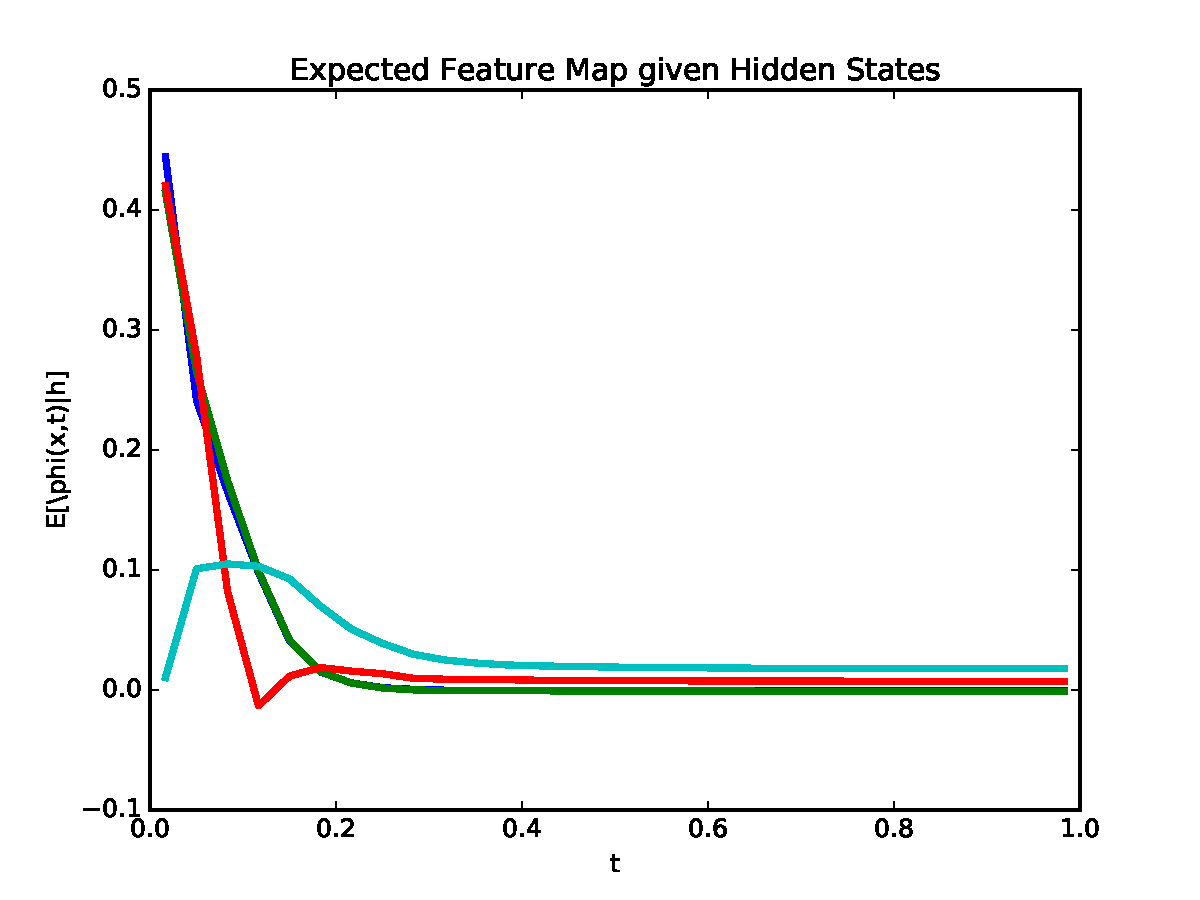
\includegraphics[width=\textwidth]{figs/vary_l/cell = E1_chr = 1_l = 20000_s = 1_m = 4_n = 30_phi = beta_full.pdf}
        \caption{$l = 20000$}
    \end{subfigure}
    \\
    \begin{subfigure}[t]{0.45\textwidth}
        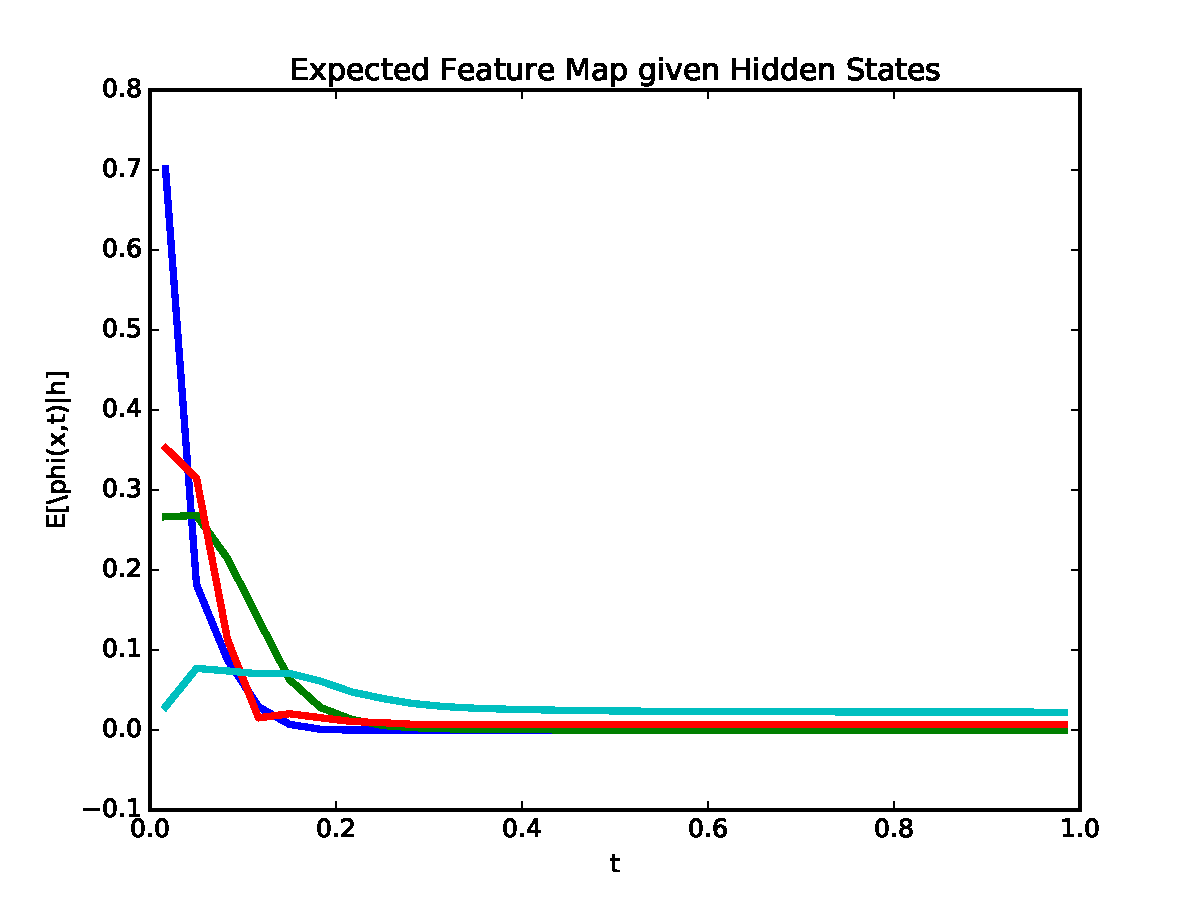
\includegraphics[width=\textwidth]{figs/vary_l/cell = E1_chr = 1_l = 40000_s = 1_m = 4_n = 30_phi = beta_full.pdf}
        \caption{$l = 40000$}
    \end{subfigure}
    &
    \begin{subfigure}[t]{0.45\textwidth}
        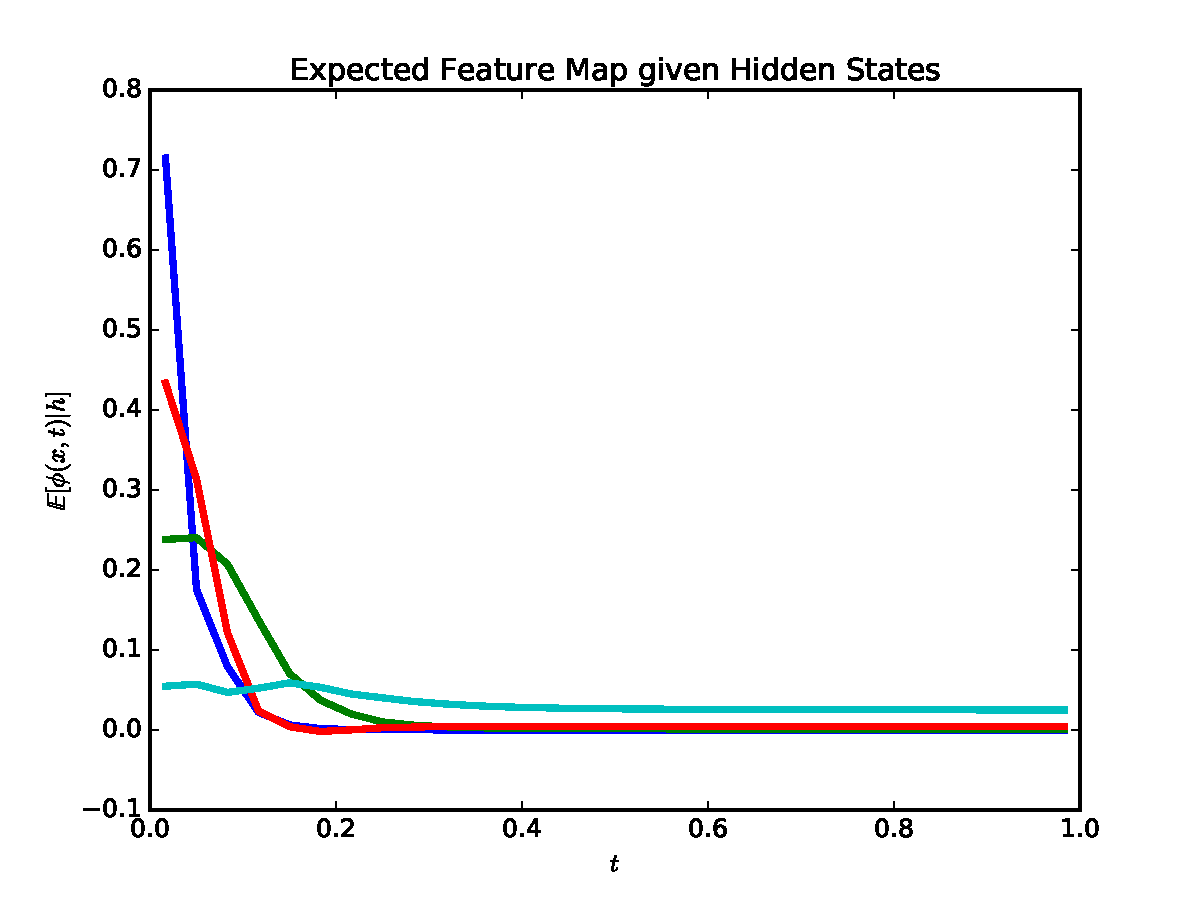
\includegraphics[width=\textwidth]{figs/vary_l/cell = E1_chr = 1_l = 80000_s = 1_m = 4_n = 30_phi = beta_full.pdf}
        \caption{$l = 80000$}
    \end{subfigure}
    \\
    \begin{subfigure}[t]{0.45\textwidth}
        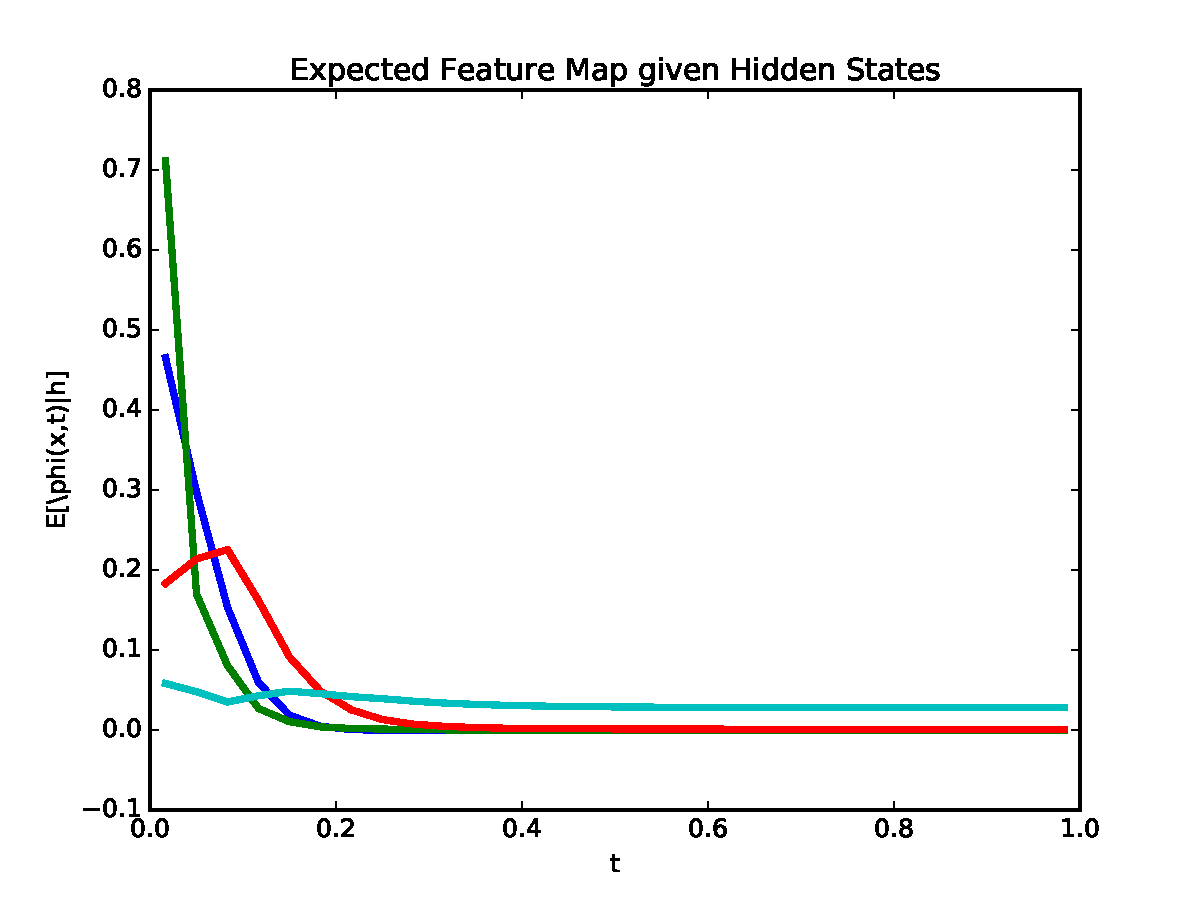
\includegraphics[width=\textwidth]{figs/vary_l/cell = E1_chr = 1_l = 160000_s = 1_m = 4_n = 30_phi = beta_full.pdf}
        \caption{$l = 160000$}
    \end{subfigure}
    &
    \begin{subfigure}[t]{0.45\textwidth}
        \includegraphics[width=\textwidth]{figs/vary_l/cell = E1_chr = 1_l = 320000_s = 1_m = 4_n = 30_phi = beta_full.pdf}
        \caption{$l = 320000$}
    \end{subfigure}
    \\
    \end{tabular}

    \caption{The observation columns of $\E[\phi(x)|h]$recovered, for varying sample size $l$. The $x$-axis is the value of $t = i/n$, the $y$-axis is the value of $(\E[\phi(x)|h])_i$.}
    \label{fig:varyl}
\end{figure}


\subsection{Effect of Specifying the Number of States}

We fix $l = 320000$, $s = 1$, and vary the number of states $m = 2,3,4,5,6,7,8,9$. Figure~\ref{fig:varym} shows the columns of $\E[\phi(x)|h]$ recovered. The spectral algorithm provides reasonable results when $m \leq 4$; when $m \geq 5$, the algorithm started to recover observation columns that has a lot of negative entries.


\begin{figure}[H]

    \begin{tabular}{cc}
    \begin{subfigure}[t]{0.45\textwidth}
        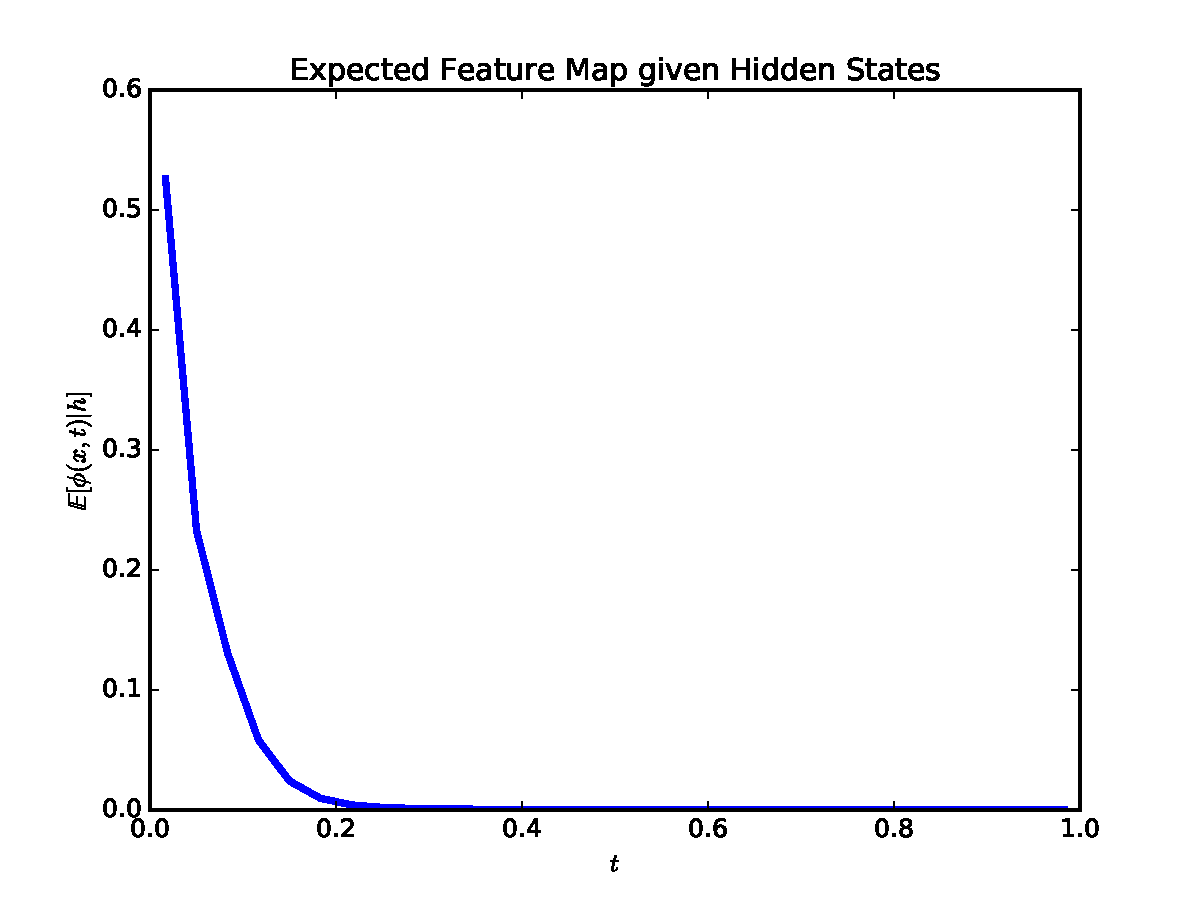
\includegraphics[width=\textwidth]{figs/vary_l/cell = E1_chr = 1_l = 320000_s = 1_m = 1_n = 30_phi = beta_full.pdf}
        \caption{$m = 1$}
    \end{subfigure}
    &
    \begin{subfigure}[t]{0.45\textwidth}
        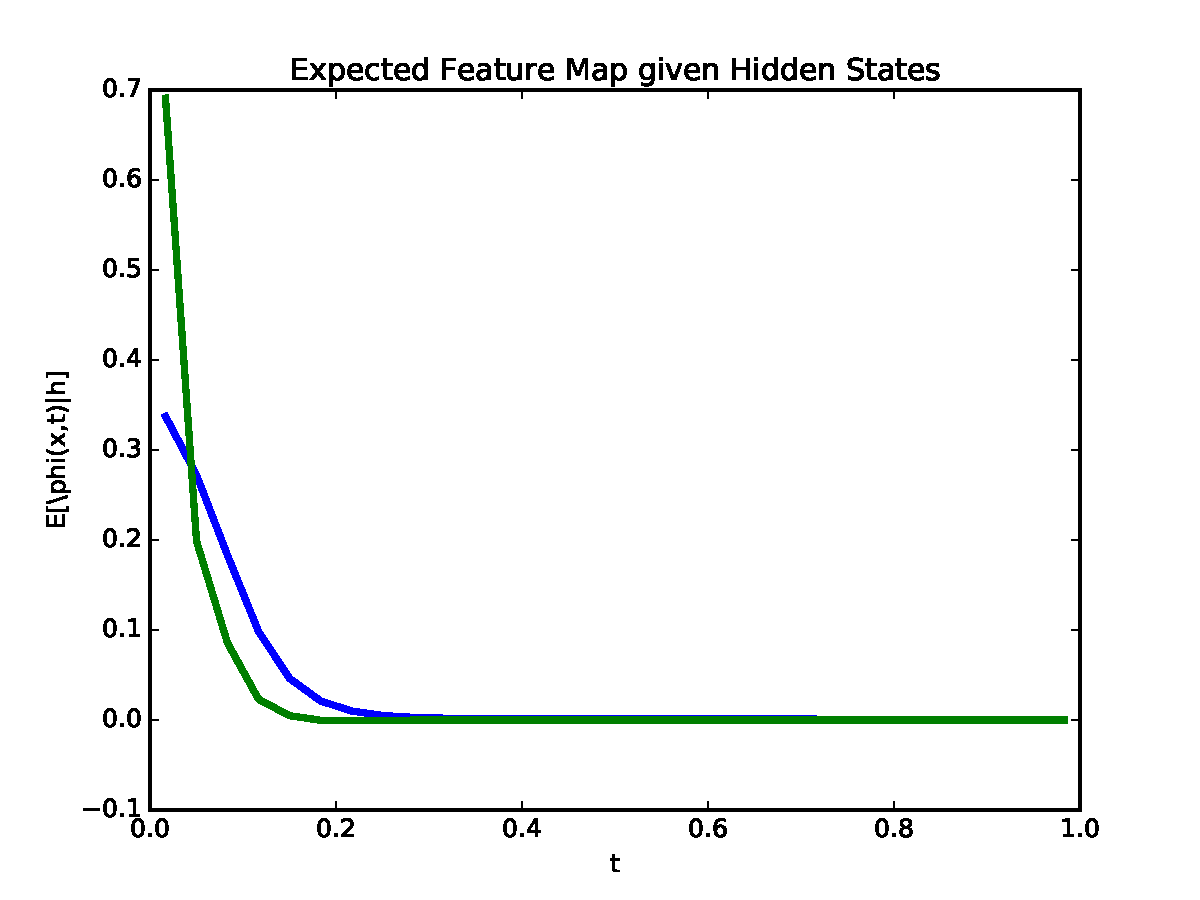
\includegraphics[width=\textwidth]{figs/vary_l/cell = E1_chr = 1_l = 320000_s = 1_m = 2_n = 30_phi = beta_full.pdf}
        \caption{$m = 2$}
    \end{subfigure}
    \\
    \begin{subfigure}[t]{0.45\textwidth}
        \includegraphics[width=\textwidth]{figs/vary_l/cell = E1_chr = 1_l = 320000_s = 1_m = 3_n = 30_phi = beta_full.pdf}
        \caption{$m = 3$}
    \end{subfigure}
    &
    \begin{subfigure}[t]{0.45\textwidth}
        \includegraphics[width=\textwidth]{figs/vary_l/cell = E1_chr = 1_l = 320000_s = 1_m = 4_n = 30_phi = beta_full.pdf}
        \caption{$m = 4$}
    \end{subfigure}
    \\
    \begin{subfigure}[t]{0.45\textwidth}
        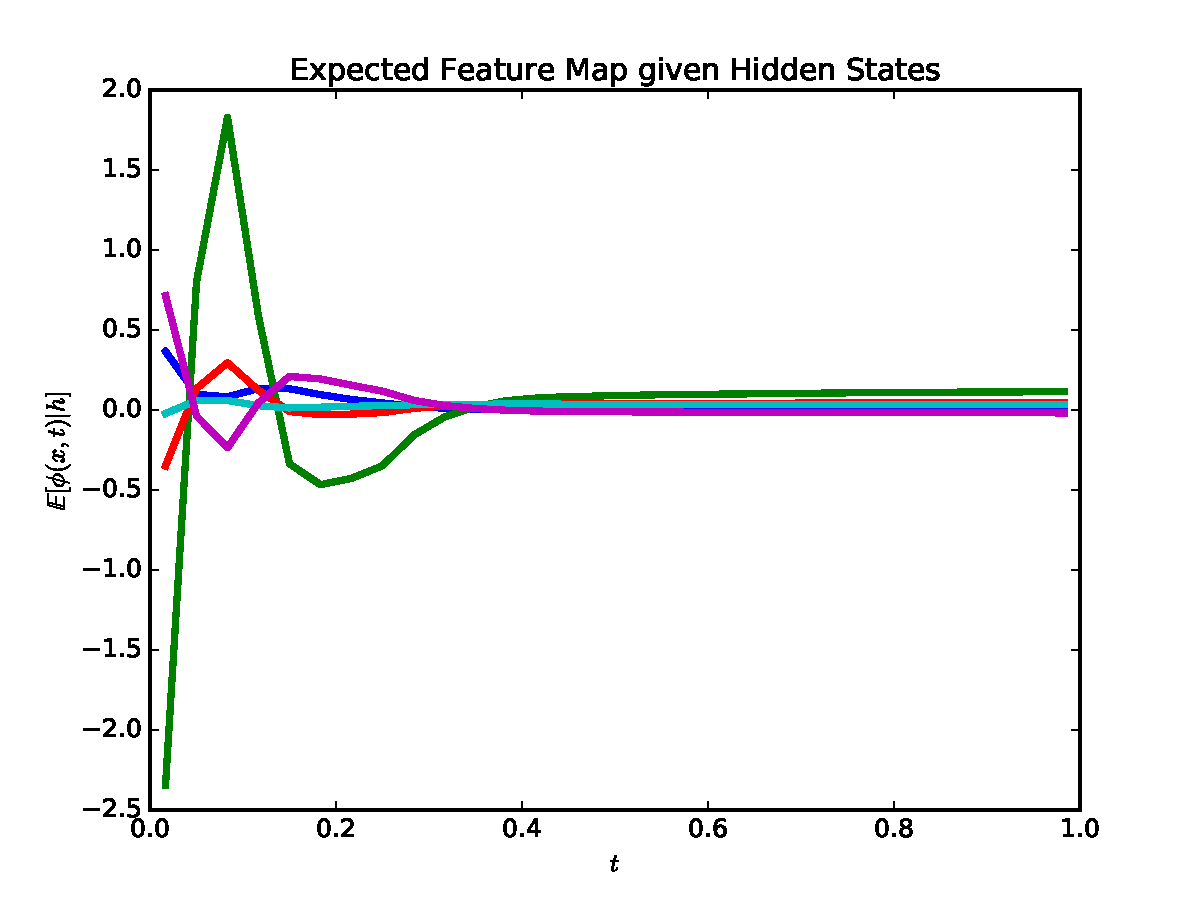
\includegraphics[width=\textwidth]{figs/vary_l/cell = E1_chr = 1_l = 320000_s = 1_m = 5_n = 30_phi = beta_full.pdf}
        \caption{$m = 5$}
    \end{subfigure}
    \end{tabular}

    \caption{The observation columns of $\E[\phi(x)|h]$recovered, for varying number of states $m$. The $x$-axis is the value of $t = i/n$, the $y$-axis is the value of $(\E[\phi(x)|h])_i$.}
    \label{fig:varym}
\end{figure}

\subsection{Binning Feature vs. Beta Feature}

We compare the experimental results using two types of feature maps $\phi_{\bin, n}$ and $\phi_{\bet, n}$. Although the two mappings are substantially different, their respective $\E[\phi(x)|h]$ have some similarities. In some sense, the beta mapping is performing a ``soft'' binning which takes into account the number count $c$ in $x$: fixing the value of methylation probability $m/c$, if $c$ is larger, then the beta mapping is closer to a binning mapping with smaller bin size. Figure~\ref{fig:varyphi} shows the columns of the recovered $\E[\phi(x)|h]$ recovered. Generally, $\phi_{\bet, n}$ produces smoother observation columns, and the results are stabler than $\phi_{\bin, n}$.

%-- double check this one experiment -- typo in file naming?

\begin{figure}[H]
    \begin{tabular}{cc}
        \begin{subfigure}[t]{0.45\textwidth}
        \includegraphics[width=\textwidth]{figs/vary_phi/cell = E1_chr = 1_l = 320000_s = 1_m = 3_n = 30_phi = beta_full.pdf}
        \caption{$\phi = \phi_{\bet, n}$ is beta mapping, $m = 3$}
    \end{subfigure}
    &
    \begin{subfigure}[t]{0.45\textwidth}
        \includegraphics[width=\textwidth]{figs/vary_phi/cell = E1_chr = 1_l = 320000_s = 1_m = 3_n = 30_phi = binning_igz.pdf}
        \caption{$\phi = \phi_{\bin, n}$ is binning mapping, $m = 3$}
    \end{subfigure}
    \\
    \begin{subfigure}[t]{0.45\textwidth}
        \includegraphics[width=\textwidth]{figs/vary_phi/cell = E1_chr = 1_l = 320000_s = 1_m = 4_n = 30_phi = beta_full.pdf}
        \caption{$\phi = \phi_{\bet, n}$ is beta mapping, $m = 4$}
    \end{subfigure}
    &
    \begin{subfigure}[t]{0.45\textwidth}
        \includegraphics[width=\textwidth]{figs/vary_phi/cell = E1_chr = 1_l = 320000_s = 1_m = 4_n = 30_phi = binning_igz.pdf}
        \caption{$\phi = \phi_{\bin, n}$ is binning mapping, $m = 4$}
    \end{subfigure}
    \end{tabular}

    \caption{The observation columns of $\E[\phi(x)|h]$recovered, for $m = 3,4$ and two types of feature map $\phi$. The $x$-axis is the value of $t = i/n$, the $y$-axis is the value of $(\E[\phi(x)|h])_i$.}
    \label{fig:varyphi}
\end{figure}

\subsection{Effect of Number of Segments Combined}
We fix $l = 320000$, $m = 4$, and vary the number of merged segments $s = 1,2,3,4,5,6,7,8$. Figure~\ref{fig:varys} shows the columns of the recovered $\E[\phi(x)|h]$. It can be seen that the recovered result is fairly insensitive to the choice of $s$.

\begin{figure}[H]
    \begin{tabular}{cc}
    \begin{subfigure}[t]{0.45\textwidth}
        \includegraphics[width=\textwidth]{figs/vary_s/cell = E1_chr = 1_l = 320000_s = 1_m = 4_n = 30_phi = beta_full.pdf}
        \caption{$s = 1$}
    \end{subfigure}
    &
    \begin{subfigure}[t]{0.45\textwidth}
        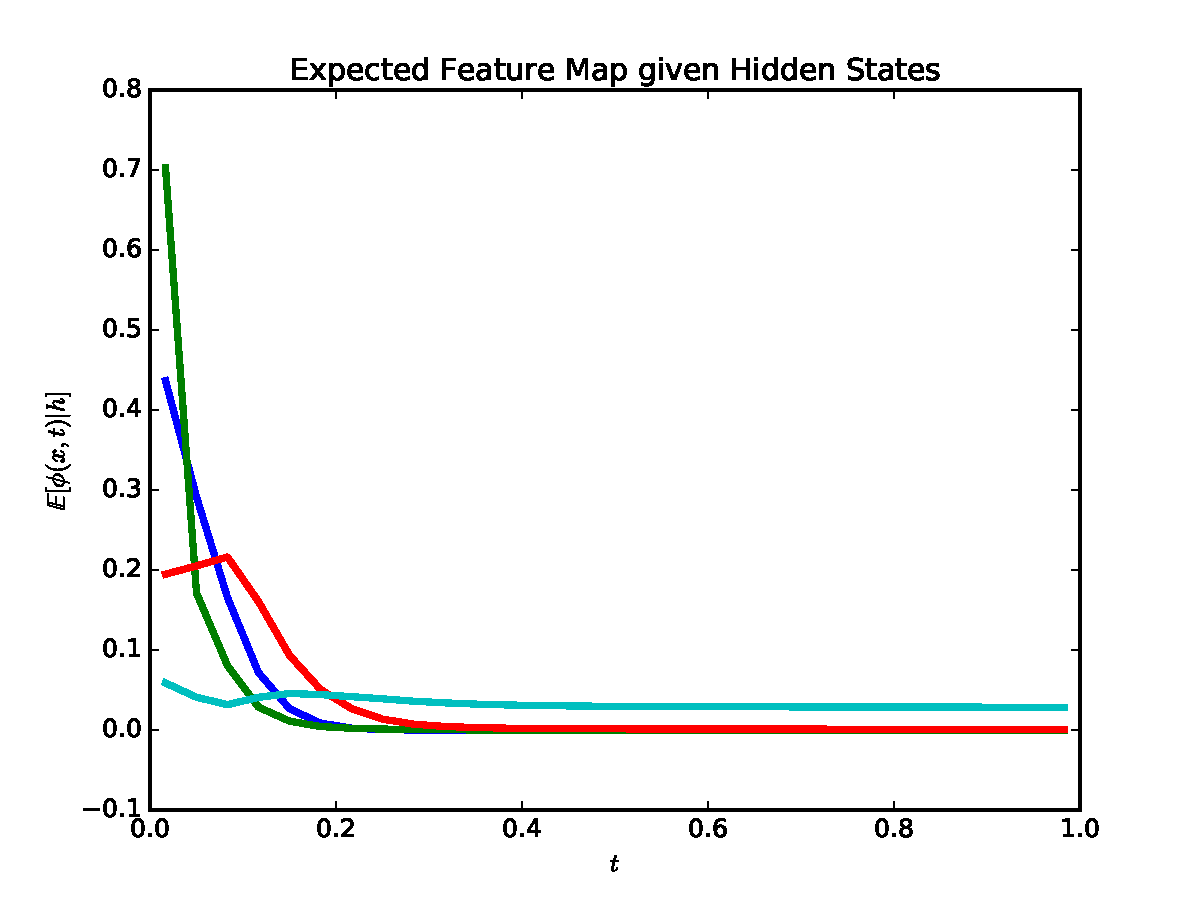
\includegraphics[width=\textwidth]{figs/vary_s/cell = E1_chr = 1_l = 320000_s = 2_m = 4_n = 30_phi = beta_full.pdf}
        \caption{$s = 2$}
    \end{subfigure}
    \\
    \begin{subfigure}[t]{0.45\textwidth}
        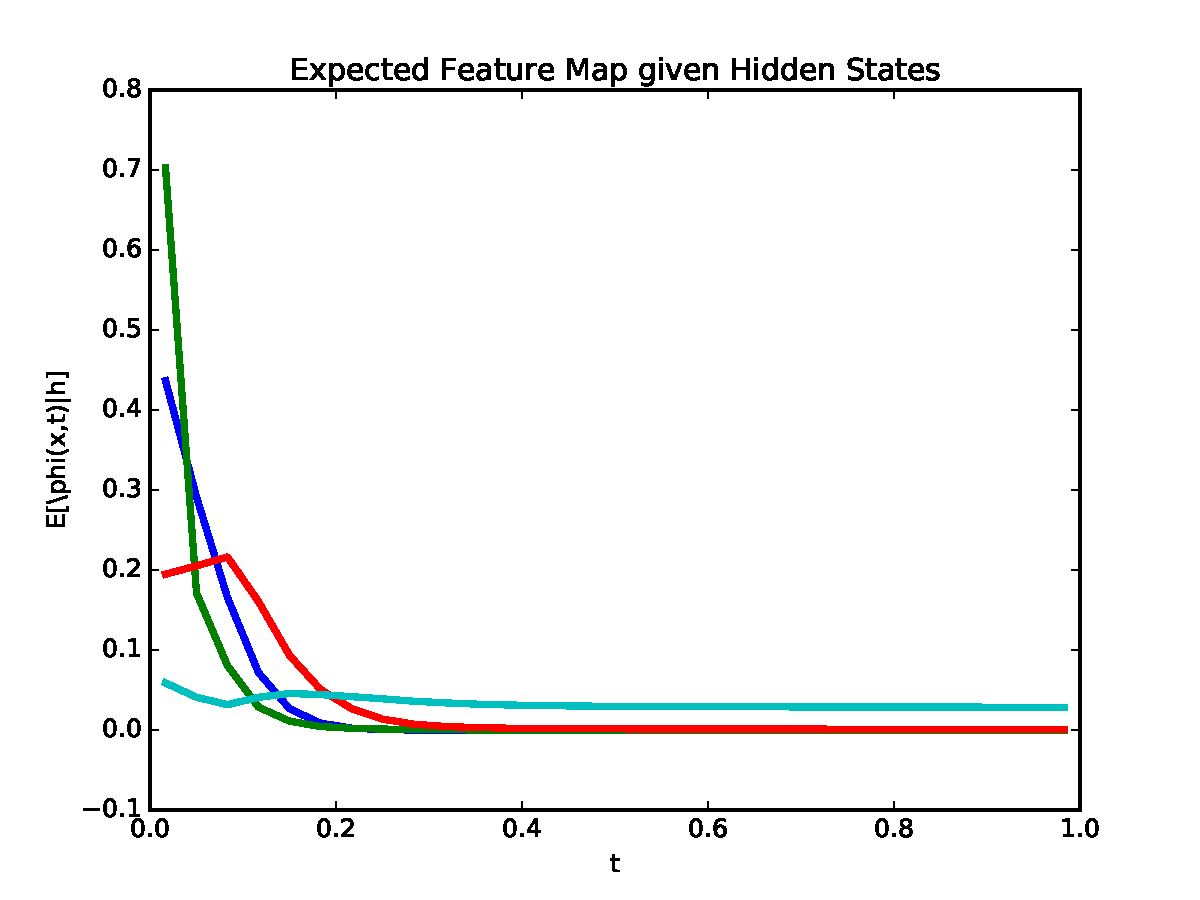
\includegraphics[width=\textwidth]{figs/vary_s/cell = E1_chr = 1_l = 320000_s = 3_m = 4_n = 30_phi = beta_full.pdf}
        \caption{$s = 3$}
    \end{subfigure}
    &
    \begin{subfigure}[t]{0.45\textwidth}
        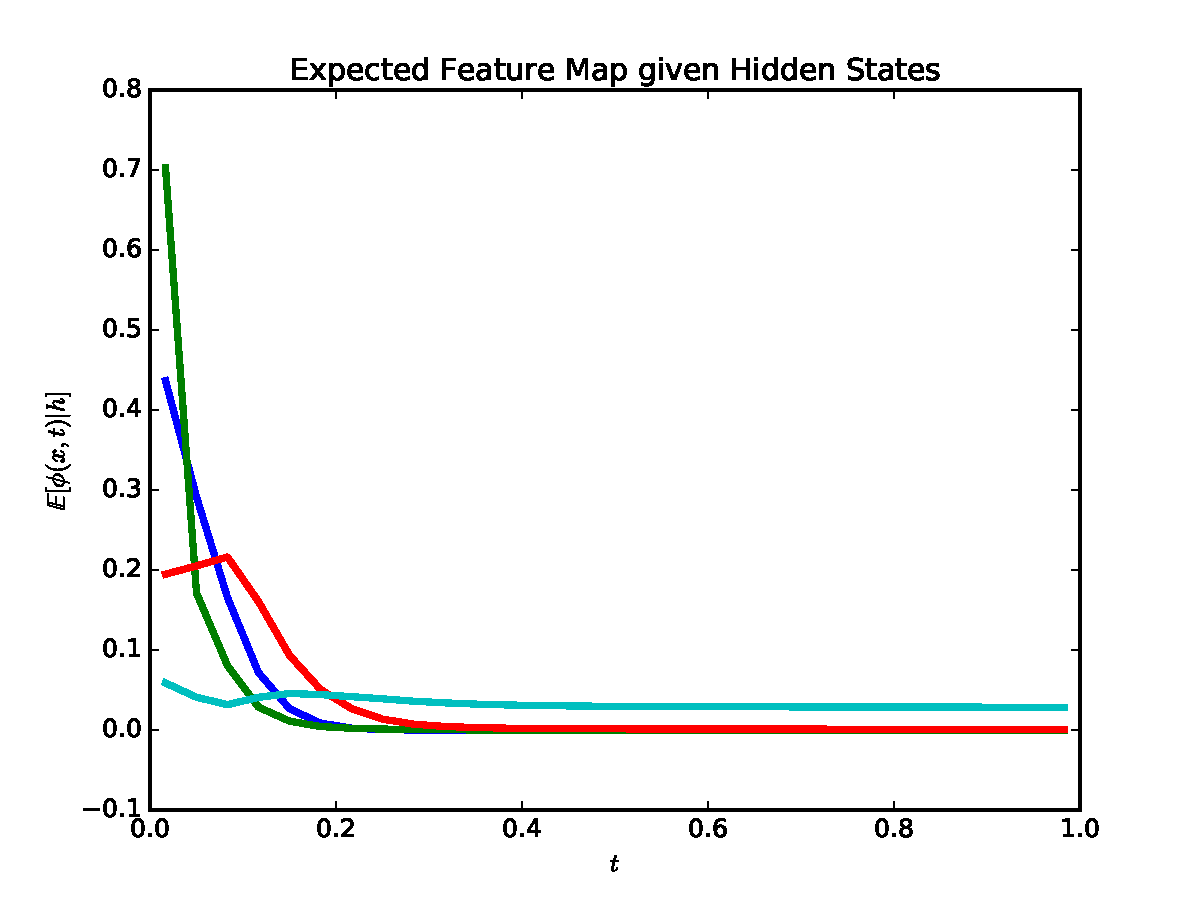
\includegraphics[width=\textwidth]{figs/vary_s/cell = E1_chr = 1_l = 320000_s = 4_m = 4_n = 30_phi = beta_full.pdf}
        \caption{$s = 4$}
    \end{subfigure}
    \\
    \begin{subfigure}[t]{0.45\textwidth}
        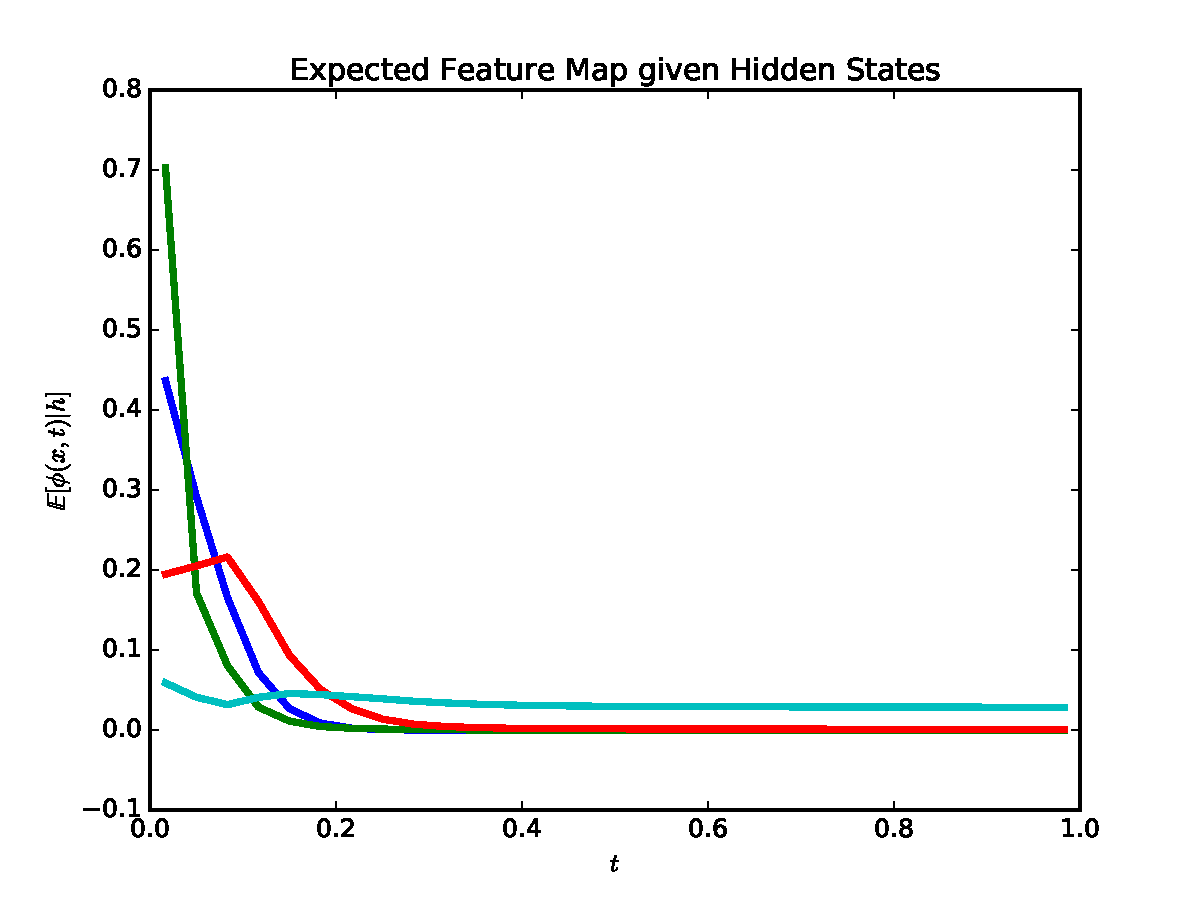
\includegraphics[width=\textwidth]{figs/vary_s/cell = E1_chr = 1_l = 320000_s = 5_m = 4_n = 30_phi = beta_full.pdf}
        \caption{$s = 5$}
    \end{subfigure}
    \end{tabular}

    \caption{The observation columns of $\E[\phi(x)|h]$recovered, for $m = 4$ and beta feature map $\phi$. The $x$-axis is the value of $t = i/n$, the $y$-axis is the value of $(\E[\phi(x)|h])_i$.}
    \label{fig:varys}
\end{figure}

\section{Experiments with CG methylations}
It is previously known that CG sites has different methylation behavior
compared to non-CG sites. We conduct experiments by merging the coverages and
the methylation counts only in contexts CGA, CGT, CGC, CGG (rows 13 to 16 of
the data).

\subsection{Effect of Number of Hidden States}
Our first set of experiments is on investigating the effect of $m$, the number of hidden
states. We vary $m$ from 1 to 8, and plot the observation matrices in
Figure~\ref{fig:varymcg}.

It can be seen from the figures below that the range of plausible $m$'s are broader:
unlike the full dataset where the observation columns start to have
large negative entries starting from $m \geq 4$, the CG subset still produces
palusible output when $m = 5,6$. In addition, some hidden states recovered
has a large methylation probability, which is not observed in the full dataset
(see e.g. Figure~\ref{fig:varym}.)

\begin{figure}[H]

    \begin{tabular}{cc}
    \begin{subfigure}[t]{0.4\textwidth}
        \includegraphics[width=\textwidth]{figs/cg/cell = E1_chr = 1_l = 320000_s = 1_m = 1_n = 50_phi = beta_full_ctxt = 12131415.pdf}
        \caption{$m = 1$}
    \end{subfigure}
    &
    \begin{subfigure}[t]{0.4\textwidth}
        \includegraphics[width=\textwidth]{figs/cg/cell = E1_chr = 1_l = 320000_s = 1_m = 2_n = 50_phi = beta_full_ctxt = 12131415.pdf}
        \caption{$m = 2$}
    \end{subfigure}
    \\
    \begin{subfigure}[t]{0.4\textwidth}
        \includegraphics[width=\textwidth]{figs/cg/cell = E1_chr = 1_l = 320000_s = 1_m = 3_n = 50_phi = beta_full_ctxt = 12131415.pdf}
        \caption{$m = 3$}
    \end{subfigure}
    &
    \begin{subfigure}[t]{0.4\textwidth}
        \includegraphics[width=\textwidth]{figs/cg/cell = E1_chr = 1_l = 320000_s = 1_m = 4_n = 50_phi = beta_full_ctxt = 12131415.pdf}
        \caption{$m = 4$}
    \end{subfigure}
    \\
    \begin{subfigure}[t]{0.4\textwidth}
        \includegraphics[width=\textwidth]{figs/cg/cell = E1_chr = 1_l = 320000_s = 1_m = 5_n = 50_phi = beta_full_ctxt = 12131415.pdf}
        \caption{$m = 5$}
    \end{subfigure}
    &
    \begin{subfigure}[t]{0.4\textwidth}
        \includegraphics[width=\textwidth]{figs/cg/cell = E1_chr = 1_l = 320000_s = 1_m = 6_n = 50_phi = beta_full_ctxt = 12131415.pdf}
        \caption{$m = 6$}
    \end{subfigure}
    \\
    \begin{subfigure}[t]{0.4\textwidth}
        \includegraphics[width=\textwidth]{figs/cg/cell = E1_chr = 1_l = 320000_s = 1_m = 7_n = 50_phi = beta_full_ctxt = 12131415.pdf}
        \caption{$m = 7$}
    \end{subfigure}
    &
    \begin{subfigure}[t]{0.4\textwidth}
        \includegraphics[width=\textwidth]{figs/cg/cell = E1_chr = 1_l = 320000_s = 1_m = 8_n = 50_phi = beta_full_ctxt = 12131415.pdf}
        \caption{$m = 8$}
    \end{subfigure}

    \end{tabular}

    \caption{The observation columns of $\E[\phi(x)|h]$recovered, for varying number of states $m$. The $x$-axis is the value of $t = i/n$, the $y$-axis is the value of $(\E[\phi(x)|h])_i$.}
    \label{fig:varymcg}
\end{figure}

\subsection{Effects of Feature Maps}
We next conduct a set of comparisons between the beta feature map and the binning
feature map, setting the dimension of feature maps $n = 50$.
It can be seen that overall, binning features produce ``rougher''
observation columns. As with the range of plausible $m$'s, binning feature performs
badly when $m \geq 5$, while beta feature consistently produces reasonable result
even if $m = 5,6$. Both approaches output nonsensical observation matrices when
$m = 7, 8$.

In addition, algorithm using the binning features cannot capture hidden states that has
low methylation probability (for all the hidden states, the conditional
methylation frequency histograms skew towards right).

\begin{figure}[H]
    \begin{tabular}{cc}
    \begin{subfigure}[t]{0.4\textwidth}
      \includegraphics[width=\textwidth]{figs/cg/cell = E1_chr = 1_l = 320000_s = 1_m = 2_n = 50_phi = beta_full_ctxt = 12131415.pdf}
      \caption{$\phi = \phi_{\bet, n}$ is beta mapping, $m = 2$}
    \end{subfigure}
    &
    \begin{subfigure}[t]{0.4\textwidth}
      \includegraphics[width=\textwidth]{figs/cg/cell = E1_chr = 1_l = 320000_s = 1_m = 2_n = 50_phi = binning_ctxt = 12131415.pdf}
      \caption{$\phi = \phi_{\bin, n}$ is binning mapping, $m = 2$}
    \end{subfigure}
    \\
    \begin{subfigure}[t]{0.4\textwidth}
        \includegraphics[width=\textwidth]{figs/cg/cell = E1_chr = 1_l = 320000_s = 1_m = 3_n = 50_phi = beta_full_ctxt = 12131415.pdf}
        \caption{$\phi = \phi_{\bet, n}$ is beta mapping, $m = 3$}
    \end{subfigure}
    &
    \begin{subfigure}[t]{0.4\textwidth}
        \includegraphics[width=\textwidth]{figs/cg/cell = E1_chr = 1_l = 320000_s = 1_m = 3_n = 50_phi = binning_ctxt = 12131415.pdf}
        \caption{$\phi = \phi_{\bin, n}$ is binning mapping, $m = 3$}
    \end{subfigure}
    \\
    \begin{subfigure}[t]{0.4\textwidth}
        \includegraphics[width=\textwidth]{figs/cg/cell = E1_chr = 1_l = 320000_s = 1_m = 4_n = 50_phi = beta_full_ctxt = 12131415.pdf}
        \caption{$\phi = \phi_{\bet, n}$ is beta mapping, $m = 4$}
    \end{subfigure}
    &
    \begin{subfigure}[t]{0.4\textwidth}
        \includegraphics[width=\textwidth]{figs/cg/cell = E1_chr = 1_l = 320000_s = 1_m = 4_n = 50_phi = binning_ctxt = 12131415.pdf}
        \caption{$\phi = \phi_{\bin, n}$ is binning mapping, $m = 4$}
    \end{subfigure}
    \\
    \begin{subfigure}[t]{0.4\textwidth}
        \includegraphics[width=\textwidth]{figs/cg/cell = E1_chr = 1_l = 320000_s = 1_m = 5_n = 50_phi = beta_full_ctxt = 12131415.pdf}
        \caption{$\phi = \phi_{\bet, n}$ is beta mapping, $m = 5$}
    \end{subfigure}
    &
    \begin{subfigure}[t]{0.4\textwidth}
        \includegraphics[width=\textwidth]{figs/cg/cell = E1_chr = 1_l = 320000_s = 1_m = 5_n = 50_phi = binning_ctxt = 12131415.pdf}
        \caption{$\phi = \phi_{\bin, n}$ is binning mapping, $m = 5$}
    \end{subfigure}
    \end{tabular}
    \caption{The observation columns of $\E[\phi(x)|h]$recovered, for $m = 2,3,4,5$ and two types of feature map $\phi$. The $x$-axis is the value of $t = i/n$, the $y$-axis is the value of $(\E[\phi(x)|h])_i$.}
    \label{fig:varyphicg}
\end{figure}

\begin{figure}[H]
    \begin{tabular}{cc}
    \begin{subfigure}[t]{0.4\textwidth}
      \includegraphics[width=\textwidth]{figs/cg/cell = E1_chr = 1_l = 320000_s = 1_m = 6_n = 50_phi = beta_full_ctxt = 12131415.pdf}
      \caption{$\phi = \phi_{\bet, n}$ is beta mapping, $m = 6$}
    \end{subfigure}
    &
    \begin{subfigure}[t]{0.4\textwidth}
      \includegraphics[width=\textwidth]{figs/cg/cell = E1_chr = 1_l = 320000_s = 1_m = 6_n = 50_phi = binning_ctxt = 12131415.pdf}
      \caption{$\phi = \phi_{\bin, n}$ is binning mapping, $m = 6$}
    \end{subfigure}
    \\
    \begin{subfigure}[t]{0.4\textwidth}
        \includegraphics[width=\textwidth]{figs/cg/cell = E1_chr = 1_l = 320000_s = 1_m = 7_n = 50_phi = beta_full_ctxt = 12131415.pdf}
        \caption{$\phi = \phi_{\bet, n}$ is beta mapping, $m = 7$}
    \end{subfigure}
    &
    \begin{subfigure}[t]{0.4\textwidth}
        \includegraphics[width=\textwidth]{figs/cg/cell = E1_chr = 1_l = 320000_s = 1_m = 7_n = 50_phi = binning_ctxt = 12131415.pdf}
        \caption{$\phi = \phi_{\bin, n}$ is binning mapping, $m = 7$}
    \end{subfigure}
    \\
    \begin{subfigure}[t]{0.4\textwidth}
        \includegraphics[width=\textwidth]{figs/cg/cell = E1_chr = 1_l = 320000_s = 1_m = 8_n = 50_phi = beta_full_ctxt = 12131415.pdf}
        \caption{$\phi = \phi_{\bet, n}$ is beta mapping, $m = 8$}
    \end{subfigure}
    &
    \begin{subfigure}[t]{0.4\textwidth}
        \includegraphics[width=\textwidth]{figs/cg/cell = E1_chr = 1_l = 320000_s = 1_m = 8_n = 50_phi = binning_ctxt = 12131415.pdf}
        \caption{$\phi = \phi_{\bin, n}$ is binning mapping, $m = 8$}
    \end{subfigure}
    \end{tabular}
    \caption{The observation columns of $\E[\phi(x)|h]$recovered, for $m = 6,7,8$ and two types of feature map $\phi$. The $x$-axis is the value of $t = i/n$, the $y$-axis is the value of $(\E[\phi(x)|h])_i$.}
    \label{fig:varyphicg2}
\end{figure}


\section{Experiments with Posterior Decoding}

With the observation matrix $\E[\phi(x)|h]$, transition matrix $T$, and initial probability $\pi$ recovered,
we apply posterior decoding to the original sequence to get estimates of hidden states in each position (every 100 base pairs).

Empirically we see the result of posterior decoding is similar to that of Viterbi decoding, therefore we present here only the results
for posterior decoding. For illustration purposes, we set the length of our test sequence to 100000; in principle it can be set arbitrarily long.
We set the size of our training set to be 320000.

Below we visualize the recovered hidden states using horizontal bar plots of different colors, each color represents a different outcome
of hidden state. On the right panel, we plot the corresponding expected feature maps of hidden states, and the colors of feature map
curves are consistent with those in the bar plot.

It can be concluded from the plots that all the sequences we are working with are dominated by a certain hidden states. We observe that the
observation matrices recovered in the CG contexts are significantly different from that of CC, CT, CA contexts. In particular, the red hidden
state in the results of CC, CT, CA contexts represents one with a low methylation probability, whereas the red hidden state in the result of CG
represents one whose methlation probablity is high.

\subsection{CC Context}

\begin{figure}[H]
    \begin{tabular}{cc}
      \begin{subfigure}[t]{0.4\textwidth}
        \includegraphics[width=\textwidth]{figs/merge_ctxts/cell = E_chr = 1_l = 320000_s = 1_m = 2_n = 40_phi = beta_full_ctxt = |0123l_test = 320000_posterior.pdf}
        \caption{Posterior Decoding for a substring of methylation of cell E, chromosome 1.}
      \end{subfigure}
      &
      \begin{subfigure}[t]{0.4\textwidth}
        \includegraphics[width=\textwidth]{figs/merge_ctxts/cell = E_chr = 1_l = 320000_s = 1_m = 2_n = 40_phi = beta_full_ctxt = |0123_feature_map.pdf}
        \caption{Expected Feature map given the hidden states}
      \end{subfigure}
      \\
      \begin{subfigure}[t]{0.4\textwidth}
        \includegraphics[width=\textwidth]{figs/merge_ctxts/cell = E_chr = 1_l = 320000_s = 1_m = 3_n = 40_phi = beta_full_ctxt = |0123l_test = 320000_posterior.pdf}
        \caption{Posterior Decoding for a substring of methylation of cell E, chromosome 1.}
      \end{subfigure}
      &
      \begin{subfigure}[t]{0.4\textwidth}
        \includegraphics[width=\textwidth]{figs/merge_ctxts/cell = E_chr = 1_l = 320000_s = 1_m = 3_n = 40_phi = beta_full_ctxt = |0123_feature_map.pdf}
        \caption{Expected Feature map given the hidden states}
      \end{subfigure}
      \\
      \begin{subfigure}[t]{0.4\textwidth}
        \includegraphics[width=\textwidth]{figs/merge_ctxts/cell = E_chr = 1_l = 320000_s = 1_m = 4_n = 40_phi = beta_full_ctxt = |0123l_test = 320000_posterior.pdf}
        \caption{Posterior Decoding for a substring of methylation of cell E, chromosome 1.}
      \end{subfigure}
      &
      \begin{subfigure}[t]{0.4\textwidth}
        \includegraphics[width=\textwidth]{figs/merge_ctxts/cell = E_chr = 1_l = 320000_s = 1_m = 4_n = 40_phi = beta_full_ctxt = |0123_feature_map.pdf}
        \caption{Expected Feature map given the hidden states}
      \end{subfigure}
    \end{tabular}
  \end{figure}


    \begin{figure}[H]
        \begin{tabular}{cc}
          \begin{subfigure}[t]{0.4\textwidth}
            \includegraphics[width=\textwidth]{figs/merge_ctxts/cell = E_chr = 1_l = 320000_s = 1_m = 5_n = 40_phi = beta_full_ctxt = |0123l_test = 320000_posterior.pdf}
            \caption{Posterior Decoding for a substring of methylation of cell E, chromosome 1.}
          \end{subfigure}
          &
          \begin{subfigure}[t]{0.4\textwidth}
            \includegraphics[width=\textwidth]{figs/merge_ctxts/cell = E_chr = 1_l = 320000_s = 1_m = 5_n = 40_phi = beta_full_ctxt = |0123_feature_map.pdf}
            \caption{Expected Feature map given the hidden states}
          \end{subfigure}
      \\
      \begin{subfigure}[t]{0.4\textwidth}
        \includegraphics[width=\textwidth]{figs/merge_ctxts/cell = E_chr = 1_l = 320000_s = 1_m = 6_n = 40_phi = beta_full_ctxt = |0123l_test = 320000_posterior.pdf}
        \caption{Posterior Decoding for a substring of methylation of cell E, chromosome 1.}
      \end{subfigure}
      &
      \begin{subfigure}[t]{0.4\textwidth}
        \includegraphics[width=\textwidth]{figs/merge_ctxts/cell = E_chr = 1_l = 320000_s = 1_m = 6_n = 40_phi = beta_full_ctxt = |0123_feature_map.pdf}
        \caption{Expected Feature map given the hidden states}
      \end{subfigure}
    \end{tabular}
\end{figure}


\subsection{CT Context}

\begin{figure}[H]
    \begin{tabular}{cc}
      \begin{subfigure}[t]{0.4\textwidth}
        \includegraphics[width=\textwidth]{figs/merge_ctxts/cell = E_chr = 1_l = 320000_s = 1_m = 2_n = 40_phi = beta_full_ctxt = |4567l_test = 320000_posterior.pdf}
        \caption{Posterior Decoding for a substring of methylation of cell E, chromosome 1.}
      \end{subfigure}
      &
      \begin{subfigure}[t]{0.4\textwidth}
        \includegraphics[width=\textwidth]{figs/merge_ctxts/cell = E_chr = 1_l = 320000_s = 1_m = 2_n = 40_phi = beta_full_ctxt = |4567_feature_map.pdf}
        \caption{Expected Feature map given the hidden states}
      \end{subfigure}
      \\
      \begin{subfigure}[t]{0.4\textwidth}
        \includegraphics[width=\textwidth]{figs/merge_ctxts/cell = E_chr = 1_l = 320000_s = 1_m = 3_n = 40_phi = beta_full_ctxt = |4567l_test = 320000_posterior.pdf}
        \caption{Posterior Decoding for a substring of methylation of cell E, chromosome 1.}
      \end{subfigure}
      &
      \begin{subfigure}[t]{0.4\textwidth}
        \includegraphics[width=\textwidth]{figs/merge_ctxts/cell = E_chr = 1_l = 320000_s = 1_m = 3_n = 40_phi = beta_full_ctxt = |4567_feature_map.pdf}
        \caption{Expected Feature map given the hidden states}
      \end{subfigure}
      \\
      \begin{subfigure}[t]{0.4\textwidth}
        \includegraphics[width=\textwidth]{figs/merge_ctxts/cell = E_chr = 1_l = 320000_s = 1_m = 4_n = 40_phi = beta_full_ctxt = |4567l_test = 320000_posterior.pdf}
        \caption{Posterior Decoding for a substring of methylation of cell E, chromosome 1.}
      \end{subfigure}
      &
      \begin{subfigure}[t]{0.4\textwidth}
        \includegraphics[width=\textwidth]{figs/merge_ctxts/cell = E_chr = 1_l = 320000_s = 1_m = 4_n = 40_phi = beta_full_ctxt = |4567_feature_map.pdf}
        \caption{Expected Feature map given the hidden states}
      \end{subfigure}
    \end{tabular}
  \end{figure}


    \begin{figure}[H]
        \begin{tabular}{cc}
          \begin{subfigure}[t]{0.4\textwidth}
            \includegraphics[width=\textwidth]{figs/merge_ctxts/cell = E_chr = 1_l = 320000_s = 1_m = 5_n = 40_phi = beta_full_ctxt = |4567l_test = 320000_posterior.pdf}
            \caption{Posterior Decoding for a substring of methylation of cell E, chromosome 1.}
          \end{subfigure}
          &
          \begin{subfigure}[t]{0.4\textwidth}
            \includegraphics[width=\textwidth]{figs/merge_ctxts/cell = E_chr = 1_l = 320000_s = 1_m = 5_n = 40_phi = beta_full_ctxt = |4567_feature_map.pdf}
            \caption{Expected Feature map given the hidden states}
          \end{subfigure}
      \\
      \begin{subfigure}[t]{0.4\textwidth}
        \includegraphics[width=\textwidth]{figs/merge_ctxts/cell = E_chr = 1_l = 320000_s = 1_m = 6_n = 40_phi = beta_full_ctxt = |4567l_test = 320000_posterior.pdf}
        \caption{Posterior Decoding for a substring of methylation of cell E, chromosome 1.}
      \end{subfigure}
      &
      \begin{subfigure}[t]{0.4\textwidth}
        \includegraphics[width=\textwidth]{figs/merge_ctxts/cell = E_chr = 1_l = 320000_s = 1_m = 6_n = 40_phi = beta_full_ctxt = |4567_feature_map.pdf}
        \caption{Expected Feature map given the hidden states}
      \end{subfigure}
    \end{tabular}
\end{figure}

\subsection{CA Context}

\begin{figure}[H]
    \begin{tabular}{cc}
      \begin{subfigure}[t]{0.4\textwidth}
        \includegraphics[width=\textwidth]{figs/merge_ctxts/cell = E_chr = 1_l = 320000_s = 1_m = 2_n = 40_phi = beta_full_ctxt = |891011l_test = 320000_posterior.pdf}
        \caption{Posterior Decoding for a substring of methylation of cell E, chromosome 1.}
      \end{subfigure}
      &
      \begin{subfigure}[t]{0.4\textwidth}
        \includegraphics[width=\textwidth]{figs/merge_ctxts/cell = E_chr = 1_l = 320000_s = 1_m = 2_n = 40_phi = beta_full_ctxt = |891011_feature_map.pdf}
        \caption{Expected Feature map given the hidden states}
      \end{subfigure}
      \\
      \begin{subfigure}[t]{0.4\textwidth}
        \includegraphics[width=\textwidth]{figs/merge_ctxts/cell = E_chr = 1_l = 320000_s = 1_m = 3_n = 40_phi = beta_full_ctxt = |891011l_test = 320000_posterior.pdf}
        \caption{Posterior Decoding for a substring of methylation of cell E, chromosome 1.}
      \end{subfigure}
      &
      \begin{subfigure}[t]{0.4\textwidth}
        \includegraphics[width=\textwidth]{figs/merge_ctxts/cell = E_chr = 1_l = 320000_s = 1_m = 3_n = 40_phi = beta_full_ctxt = |891011_feature_map.pdf}
        \caption{Expected Feature map given the hidden states}
      \end{subfigure}
      \\
      \begin{subfigure}[t]{0.4\textwidth}
        \includegraphics[width=\textwidth]{figs/merge_ctxts/cell = E_chr = 1_l = 320000_s = 1_m = 4_n = 40_phi = beta_full_ctxt = |891011l_test = 320000_posterior.pdf}
        \caption{Posterior Decoding for a substring of methylation of cell E, chromosome 1.}
      \end{subfigure}
      &
      \begin{subfigure}[t]{0.4\textwidth}
        \includegraphics[width=\textwidth]{figs/merge_ctxts/cell = E_chr = 1_l = 320000_s = 1_m = 4_n = 40_phi = beta_full_ctxt = |891011_feature_map.pdf}
        \caption{Expected Feature map given the hidden states}
      \end{subfigure}
    \end{tabular}
  \end{figure}


    \begin{figure}[H]
        \begin{tabular}{cc}
          \begin{subfigure}[t]{0.4\textwidth}
            \includegraphics[width=\textwidth]{figs/merge_ctxts/cell = E_chr = 1_l = 320000_s = 1_m = 5_n = 40_phi = beta_full_ctxt = |891011l_test = 320000_posterior.pdf}
            \caption{Posterior Decoding for a substring of methylation of cell E, chromosome 1.}
          \end{subfigure}
          &
          \begin{subfigure}[t]{0.4\textwidth}
            \includegraphics[width=\textwidth]{figs/merge_ctxts/cell = E_chr = 1_l = 320000_s = 1_m = 5_n = 40_phi = beta_full_ctxt = |891011_feature_map.pdf}
            \caption{Expected Feature map given the hidden states}
          \end{subfigure}
      \\
      \begin{subfigure}[t]{0.4\textwidth}
        \includegraphics[width=\textwidth]{figs/merge_ctxts/cell = E_chr = 1_l = 320000_s = 1_m = 6_n = 40_phi = beta_full_ctxt = |891011l_test = 320000_posterior.pdf}
        \caption{Posterior Decoding for a substring of methylation of cell E, chromosome 1.}
      \end{subfigure}
      &
      \begin{subfigure}[t]{0.4\textwidth}
        \includegraphics[width=\textwidth]{figs/merge_ctxts/cell = E_chr = 1_l = 320000_s = 1_m = 6_n = 40_phi = beta_full_ctxt = |891011_feature_map.pdf}
        \caption{Expected Feature map given the hidden states}
      \end{subfigure}
    \end{tabular}
\end{figure}

\subsection{CG Context}

\begin{figure}[H]
    \begin{tabular}{cc}
      \begin{subfigure}[t]{0.4\textwidth}
        \includegraphics[width=\textwidth]{figs/merge_ctxts/cell = E_chr = 1_l = 320000_s = 1_m = 2_n = 40_phi = beta_full_ctxt = |12131415l_test = 320000_posterior.pdf}
        \caption{Posterior Decoding for a substring of methylation of cell E, chromosome 1.}
      \end{subfigure}
      &
      \begin{subfigure}[t]{0.4\textwidth}
        \includegraphics[width=\textwidth]{figs/merge_ctxts/cell = E_chr = 1_l = 320000_s = 1_m = 2_n = 40_phi = beta_full_ctxt = |12131415_feature_map.pdf}
        \caption{Expected Feature map given the hidden states}
      \end{subfigure}
      \\
      \begin{subfigure}[t]{0.4\textwidth}
        \includegraphics[width=\textwidth]{figs/merge_ctxts/cell = E_chr = 1_l = 320000_s = 1_m = 3_n = 40_phi = beta_full_ctxt = |12131415l_test = 320000_posterior.pdf}
        \caption{Posterior Decoding for a substring of methylation of cell E, chromosome 1.}
      \end{subfigure}
      &
      \begin{subfigure}[t]{0.4\textwidth}
        \includegraphics[width=\textwidth]{figs/merge_ctxts/cell = E_chr = 1_l = 320000_s = 1_m = 3_n = 40_phi = beta_full_ctxt = |12131415_feature_map.pdf}
        \caption{Expected Feature map given the hidden states}
      \end{subfigure}
      \\
      \begin{subfigure}[t]{0.4\textwidth}
        \includegraphics[width=\textwidth]{figs/merge_ctxts/cell = E_chr = 1_l = 320000_s = 1_m = 4_n = 40_phi = beta_full_ctxt = |12131415l_test = 320000_posterior.pdf}
        \caption{Posterior Decoding for a substring of methylation of cell E, chromosome 1.}
      \end{subfigure}
      &
      \begin{subfigure}[t]{0.4\textwidth}
        \includegraphics[width=\textwidth]{figs/merge_ctxts/cell = E_chr = 1_l = 320000_s = 1_m = 4_n = 40_phi = beta_full_ctxt = |12131415_feature_map.pdf}
        \caption{Expected Feature map given the hidden states}
      \end{subfigure}
    \end{tabular}
  \end{figure}


    \begin{figure}[H]
        \begin{tabular}{cc}
          \begin{subfigure}[t]{0.4\textwidth}
            \includegraphics[width=\textwidth]{figs/merge_ctxts/cell = E_chr = 1_l = 320000_s = 1_m = 5_n = 40_phi = beta_full_ctxt = |12131415l_test = 320000_posterior.pdf}
            \caption{Posterior Decoding for a substring of methylation of cell E, chromosome 1.}
          \end{subfigure}
          &
          \begin{subfigure}[t]{0.4\textwidth}
            \includegraphics[width=\textwidth]{figs/merge_ctxts/cell = E_chr = 1_l = 320000_s = 1_m = 5_n = 40_phi = beta_full_ctxt = |12131415_feature_map.pdf}
            \caption{Expected Feature map given the hidden states}
          \end{subfigure}
      \\
      \begin{subfigure}[t]{0.4\textwidth}
        \includegraphics[width=\textwidth]{figs/merge_ctxts/cell = E_chr = 1_l = 320000_s = 1_m = 6_n = 40_phi = beta_full_ctxt = |12131415l_test = 320000_posterior.pdf}
        \caption{Posterior Decoding for a substring of methylation of cell E, chromosome 1.}
      \end{subfigure}
      &
      \begin{subfigure}[t]{0.4\textwidth}
        \includegraphics[width=\textwidth]{figs/merge_ctxts/cell = E_chr = 1_l = 320000_s = 1_m = 6_n = 40_phi = beta_full_ctxt = |12131415_feature_map.pdf}
        \caption{Expected Feature map given the hidden states}
      \end{subfigure}
    \end{tabular}
\end{figure}

\subsection{All Contexts}

\begin{figure}[H]
    \begin{tabular}{cc}
      \begin{subfigure}[t]{0.4\textwidth}
        \includegraphics[width=\textwidth]{figs/merge_ctxts/cell = E_chr = 1_l = 320000_s = 1_m = 2_n = 40_phi = beta_full_ctxt = |0123456789101112131415l_test = 320000_posterior.pdf}
        \caption{Posterior Decoding for a substring of methylation of cell E, chromosome 1.}
      \end{subfigure}
      &
      \begin{subfigure}[t]{0.4\textwidth}
        \includegraphics[width=\textwidth]{figs/merge_ctxts/cell = E_chr = 1_l = 320000_s = 1_m = 3_n = 40_phi = beta_full_ctxt = |0123456789101112131415_feature_map.pdf}
        \caption{Expected Feature map given the hidden states}
      \end{subfigure}
      \\
      \begin{subfigure}[t]{0.4\textwidth}
        \includegraphics[width=\textwidth]{figs/merge_ctxts/cell = E_chr = 1_l = 320000_s = 1_m = 3_n = 40_phi = beta_full_ctxt = |0123456789101112131415l_test = 320000_posterior.pdf}
        \caption{Posterior Decoding for a substring of methylation of cell E, chromosome 1.}
      \end{subfigure}
      &
      \begin{subfigure}[t]{0.4\textwidth}
        \includegraphics[width=\textwidth]{figs/merge_ctxts/cell = E_chr = 1_l = 320000_s = 1_m = 3_n = 40_phi = beta_full_ctxt = |0123456789101112131415_feature_map.pdf}
        \caption{Expected Feature map given the hidden states}
      \end{subfigure}
      \\
      \begin{subfigure}[t]{0.4\textwidth}
        \includegraphics[width=\textwidth]{figs/merge_ctxts/cell = E_chr = 1_l = 320000_s = 1_m = 4_n = 40_phi = beta_full_ctxt = |0123456789101112131415l_test = 320000_posterior.pdf}
        \caption{Posterior Decoding for a substring of methylation of cell E, chromosome 1.}
      \end{subfigure}
      &
      \begin{subfigure}[t]{0.4\textwidth}
        \includegraphics[width=\textwidth]{figs/merge_ctxts/cell = E_chr = 1_l = 320000_s = 1_m = 4_n = 40_phi = beta_full_ctxt = |0123456789101112131415_feature_map.pdf}
        \caption{Expected Feature map given the hidden states}
      \end{subfigure}
  \end{tabular}
\end{figure}


  \begin{figure}[H]
      \begin{tabular}{cc}
        \begin{subfigure}[t]{0.4\textwidth}
          \includegraphics[width=\textwidth]{figs/merge_ctxts/cell = E_chr = 1_l = 320000_s = 1_m = 5_n = 40_phi = beta_full_ctxt = |0123456789101112131415l_test = 320000_posterior.pdf}
          \caption{Posterior Decoding for a substring of methylation of cell E, chromosome 1.}
        \end{subfigure}
        &
        \begin{subfigure}[t]{0.4\textwidth}
          \includegraphics[width=\textwidth]{figs/merge_ctxts/cell = E_chr = 1_l = 320000_s = 1_m = 5_n = 40_phi = beta_full_ctxt = |0123456789101112131415_feature_map.pdf}
          \caption{Expected Feature map given the hidden states}
        \end{subfigure}
      \\
      \begin{subfigure}[t]{0.4\textwidth}
        \includegraphics[width=\textwidth]{figs/merge_ctxts/cell = E_chr = 1_l = 320000_s = 1_m = 6_n = 40_phi = beta_full_ctxt = |0123456789101112131415l_test = 320000_posterior.pdf}
        \caption{Posterior Decoding for a substring of methylation of cell E, chromosome 1.}
      \end{subfigure}
      &
      \begin{subfigure}[t]{0.4\textwidth}
        \includegraphics[width=\textwidth]{figs/merge_ctxts/cell = E_chr = 1_l = 320000_s = 1_m = 6_n = 40_phi = beta_full_ctxt = |0123456789101112131415_feature_map.pdf}
        \caption{Expected Feature map given the hidden states}
      \end{subfigure}
    \end{tabular}
\end{figure}

\section{Merging the Contexts using Conditional Independence}

We concatenate the feature representations in constexts CC, CA, CT and CG. For each
context, the dimension is 10; hence in total the feature map is of 40 dimensions.
Moreover, when performing posterior decoding, we assume the the observations are
conditionally independent, that is, for all $i$, the observation probabililty satisfies
\begin{eqnarray*}
  &&\Pr[(m_t^{CC}, m_t^{CA}, m_t^{CT}, m_t^{CG}) | c_t^{CC}, c_t^{CA}, c_t^{CT}, c_t^{CG}, h_t = i] \\
  &=&
  \Pr[m_t^{CC} | c_t^{CC}, h_t = i] \Pr[m_t^{CA} | c_t^{CA}, h_t = i] \Pr[m_t^{CT} | c_t^{CT}, h_t = i] \Pr[m_t^{CG} | c_t^{CG}, h_t = i]
\end{eqnarray*}

From the experiments below, we can see that the recovered hidden states are diverse,
and corresponds to different methylation behaviors in different contexts.


\subsection{Cell type E sequences(E1 and E2)}
\begin{figure}[H]
    \begin{tabular}{cc}
      \begin{subfigure}[t]{0.4\textwidth}
        \includegraphics[width=\textwidth]{figs/merge_ctxts/cell = E_chr = 1_l = 320000_s = 1_m = 2_n = 40_phi = beta_full_ctxt = |0123|4567|891011|12131415l_test = 320000_posterior.pdf}
        \caption{Posterior Decoding for a substring of methylation of cell E, chromosome 1.}
      \end{subfigure}
      &
      \begin{subfigure}[t]{0.6\textwidth}
        \includegraphics[width=\textwidth]{figs/merge_ctxts/cell = E_chr = 1_l = 320000_s = 1_m = 2_n = 40_phi = beta_full_ctxt = |0123|4567|891011|12131415_feature_map.pdf}
        \caption{Expected Feature map given the hidden states}
      \end{subfigure}
      \\
      \begin{subfigure}[t]{0.4\textwidth}
        \includegraphics[width=\textwidth]{figs/merge_ctxts/cell = E_chr = 1_l = 320000_s = 1_m = 3_n = 40_phi = beta_full_ctxt = |0123|4567|891011|12131415l_test = 320000_posterior.pdf}
        \caption{Posterior Decoding for a substring of methylation of cell E, chromosome 1.}
      \end{subfigure}
      &
      \begin{subfigure}[t]{0.6\textwidth}
        \includegraphics[width=\textwidth]{figs/merge_ctxts/cell = E_chr = 1_l = 320000_s = 1_m = 3_n = 40_phi = beta_full_ctxt = |0123|4567|891011|12131415_feature_map.pdf}
        \caption{Expected Feature map given the hidden states}
      \end{subfigure}
      \\
      \begin{subfigure}[t]{0.4\textwidth}
        \includegraphics[width=\textwidth]{figs/merge_ctxts/cell = E_chr = 1_l = 320000_s = 1_m = 4_n = 40_phi = beta_full_ctxt = |0123|4567|891011|12131415l_test = 320000_posterior.pdf}
        \caption{Posterior Decoding for a substring of methylation of cell E, chromosome 1.}
      \end{subfigure}
      &
      \begin{subfigure}[t]{0.6\textwidth}
        \includegraphics[width=\textwidth]{figs/merge_ctxts/cell = E_chr = 1_l = 320000_s = 1_m = 4_n = 40_phi = beta_full_ctxt = |0123|4567|891011|12131415_feature_map.pdf}
        \caption{Expected Feature map given the hidden states}
      \end{subfigure}
  \end{tabular}
\end{figure}

\begin{figure}[H]
    \begin{tabular}{cc}
      \begin{subfigure}[t]{0.4\textwidth}
        \includegraphics[width=\textwidth]{figs/merge_ctxts/cell = E_chr = 1_l = 320000_s = 1_m = 5_n = 40_phi = beta_full_ctxt = |0123|4567|891011|12131415l_test = 320000_posterior.pdf}
        \caption{Posterior Decoding for a substring of methylation of cell E, chromosome 1.}
      \end{subfigure}
      &
      \begin{subfigure}[t]{0.6\textwidth}
        \includegraphics[width=\textwidth]{figs/merge_ctxts/cell = E_chr = 1_l = 320000_s = 1_m = 5_n = 40_phi = beta_full_ctxt = |0123|4567|891011|12131415_feature_map.pdf}
        \caption{Expected Feature map given the hidden states}
      \end{subfigure}
      \\
      \begin{subfigure}[t]{0.4\textwidth}
        \includegraphics[width=\textwidth]{figs/merge_ctxts/cell = E_chr = 1_l = 320000_s = 1_m = 6_n = 40_phi = beta_full_ctxt = |0123|4567|891011|12131415l_test = 320000_posterior.pdf}
        \caption{Posterior Decoding for a substring of methylation of cell E, chromosome 1.}
      \end{subfigure}
      &
      \begin{subfigure}[t]{0.6\textwidth}
        \includegraphics[width=\textwidth]{figs/merge_ctxts/cell = E_chr = 1_l = 320000_s = 1_m = 6_n = 40_phi = beta_full_ctxt = |0123|4567|891011|12131415_feature_map.pdf}
        \caption{Expected Feature map given the hidden states}
      \end{subfigure}
  \end{tabular}
\end{figure}


\subsection{Cell type V (sequences V8 and V9)}
\begin{figure}[H]
    \begin{tabular}{cc}
      \begin{subfigure}[t]{0.4\textwidth}
        \includegraphics[width=\textwidth]{figs/merge_ctxts/cell = V_chr = 1_l = 320000_s = 1_m = 2_n = 40_phi = beta_full_ctxt = |0123|4567|891011|12131415l_test = 320000_posterior.pdf}
        \caption{Posterior Decoding for a substring of methylation of cell V, chromosome 1.}
      \end{subfigure}
      &
      \begin{subfigure}[t]{0.6\textwidth}
        \includegraphics[width=\textwidth]{figs/merge_ctxts/cell = V_chr = 1_l = 320000_s = 1_m = 2_n = 40_phi = beta_full_ctxt = |0123|4567|891011|12131415_feature_map.pdf}
        \caption{Expected Feature map given the hidden states}
      \end{subfigure}
      \\
      \begin{subfigure}[t]{0.4\textwidth}
        \includegraphics[width=\textwidth]{figs/merge_ctxts/cell = V_chr = 1_l = 320000_s = 1_m = 3_n = 40_phi = beta_full_ctxt = |0123|4567|891011|12131415l_test = 320000_posterior.pdf}
        \caption{Posterior Decoding for a substring of methylation of cell V, chromosome 1.}
      \end{subfigure}
      &
      \begin{subfigure}[t]{0.6\textwidth}
        \includegraphics[width=\textwidth]{figs/merge_ctxts/cell = V_chr = 1_l = 320000_s = 1_m = 3_n = 40_phi = beta_full_ctxt = |0123|4567|891011|12131415_feature_map.pdf}
        \caption{Expected Feature map given the hidden states}
      \end{subfigure}
      \\
      \begin{subfigure}[t]{0.4\textwidth}
        \includegraphics[width=\textwidth]{figs/merge_ctxts/cell = V_chr = 1_l = 320000_s = 1_m = 4_n = 40_phi = beta_full_ctxt = |0123|4567|891011|12131415l_test = 320000_posterior.pdf}
        \caption{Posterior Decoding for a substring of methylation of cell V, chromosome 1.}
      \end{subfigure}
      &
      \begin{subfigure}[t]{0.6\textwidth}
        \includegraphics[width=\textwidth]{figs/merge_ctxts/cell = V_chr = 1_l = 320000_s = 1_m = 4_n = 40_phi = beta_full_ctxt = |0123|4567|891011|12131415_feature_map.pdf}
        \caption{Expected Feature map given the hidden states}
      \end{subfigure}
  \end{tabular}
\end{figure}

\begin{figure}[H]
    \begin{tabular}{cc}
      \begin{subfigure}[t]{0.4\textwidth}
        \includegraphics[width=\textwidth]{figs/merge_ctxts/cell = V_chr = 1_l = 320000_s = 1_m = 5_n = 40_phi = beta_full_ctxt = |0123|4567|891011|12131415l_test = 320000_posterior.pdf}
        \caption{Posterior Decoding for a substring of methylation of cell V, chromosome 1.}
      \end{subfigure}
      &
      \begin{subfigure}[t]{0.6\textwidth}
        \includegraphics[width=\textwidth]{figs/merge_ctxts/cell = V_chr = 1_l = 320000_s = 1_m = 5_n = 40_phi = beta_full_ctxt = |0123|4567|891011|12131415_feature_map.pdf}
        \caption{Expected Feature map given the hidden states}
      \end{subfigure}
      \\
      \begin{subfigure}[t]{0.4\textwidth}
        \includegraphics[width=\textwidth]{figs/merge_ctxts/cell = V_chr = 1_l = 320000_s = 1_m = 6_n = 40_phi = beta_full_ctxt = |0123|4567|891011|12131415l_test = 320000_posterior.pdf}
        \caption{Posterior Decoding for a substring of methylation of cell V, chromosome 1.}
      \end{subfigure}
      &
      \begin{subfigure}[t]{0.6\textwidth}
        \includegraphics[width=\textwidth]{figs/merge_ctxts/cell = V_chr = 1_l = 320000_s = 1_m = 6_n = 40_phi = beta_full_ctxt = |0123|4567|891011|12131415_feature_map.pdf}
        \caption{Expected Feature map given the hidden states}
      \end{subfigure}
  \end{tabular}
\end{figure}


\subsection{Cell type P (sequences P13P14 and P15P16)}
\begin{figure}[H]
    \begin{tabular}{cc}
      \begin{subfigure}[t]{0.4\textwidth}
        \includegraphics[width=\textwidth]{figs/merge_ctxts/cell = P_chr = 1_l = 320000_s = 1_m = 2_n = 40_phi = beta_full_ctxt = |0123|4567|891011|12131415l_test = 320000_posterior.pdf}
        \caption{Posterior Decoding for a substring of methylation of cell P, chromosome 1.}
      \end{subfigure}
      &
      \begin{subfigure}[t]{0.6\textwidth}
        \includegraphics[width=\textwidth]{figs/merge_ctxts/cell = P_chr = 1_l = 320000_s = 1_m = 2_n = 40_phi = beta_full_ctxt = |0123|4567|891011|12131415_feature_map.pdf}
        \caption{Expected Feature map given the hidden states}
      \end{subfigure}
      \\
      \begin{subfigure}[t]{0.4\textwidth}
        \includegraphics[width=\textwidth]{figs/merge_ctxts/cell = P_chr = 1_l = 320000_s = 1_m = 3_n = 40_phi = beta_full_ctxt = |0123|4567|891011|12131415l_test = 320000_posterior.pdf}
        \caption{Posterior Decoding for a substring of methylation of cell P, chromosome 1.}
      \end{subfigure}
      &
      \begin{subfigure}[t]{0.6\textwidth}
        \includegraphics[width=\textwidth]{figs/merge_ctxts/cell = P_chr = 1_l = 320000_s = 1_m = 3_n = 40_phi = beta_full_ctxt = |0123|4567|891011|12131415_feature_map.pdf}
        \caption{Expected Feature map given the hidden states}
      \end{subfigure}
      \\
      \begin{subfigure}[t]{0.4\textwidth}
        \includegraphics[width=\textwidth]{figs/merge_ctxts/cell = P_chr = 1_l = 320000_s = 1_m = 4_n = 40_phi = beta_full_ctxt = |0123|4567|891011|12131415l_test = 320000_posterior.pdf}
        \caption{Posterior Decoding for a substring of methylation of cell P, chromosome 1.}
      \end{subfigure}
      &
      \begin{subfigure}[t]{0.6\textwidth}
        \includegraphics[width=\textwidth]{figs/merge_ctxts/cell = P_chr = 1_l = 320000_s = 1_m = 4_n = 40_phi = beta_full_ctxt = |0123|4567|891011|12131415_feature_map.pdf}
        \caption{Expected Feature map given the hidden states}
      \end{subfigure}
  \end{tabular}
\end{figure}

\begin{figure}[H]
    \begin{tabular}{cc}
      \begin{subfigure}[t]{0.4\textwidth}
        \includegraphics[width=\textwidth]{figs/merge_ctxts/cell = P_chr = 1_l = 320000_s = 1_m = 5_n = 40_phi = beta_full_ctxt = |0123|4567|891011|12131415l_test = 320000_posterior.pdf}
        \caption{Posterior Decoding for a substring of methylation of cell P, chromosome 1.}
      \end{subfigure}
      &
      \begin{subfigure}[t]{0.6\textwidth}
        \includegraphics[width=\textwidth]{figs/merge_ctxts/cell = P_chr = 1_l = 320000_s = 1_m = 5_n = 40_phi = beta_full_ctxt = |0123|4567|891011|12131415_feature_map.pdf}
        \caption{Expected Feature map given the hidden states}
      \end{subfigure}
      \\
      \begin{subfigure}[t]{0.4\textwidth}
        \includegraphics[width=\textwidth]{figs/merge_ctxts/cell = P_chr = 1_l = 320000_s = 1_m = 6_n = 40_phi = beta_full_ctxt = |0123|4567|891011|12131415l_test = 320000_posterior.pdf}
        \caption{Posterior Decoding for a substring of methylation of cell P, chromosome 1.}
      \end{subfigure}
      &
      \begin{subfigure}[t]{0.6\textwidth}
        \includegraphics[width=\textwidth]{figs/merge_ctxts/cell = P_chr = 1_l = 320000_s = 1_m = 6_n = 40_phi = beta_full_ctxt = |0123|4567|891011|12131415_feature_map.pdf}
        \caption{Expected Feature map given the hidden states}
      \end{subfigure}
  \end{tabular}
\end{figure}

\end{document}
